\documentclass[12pt,letterpaper]{article}

\usepackage[top=2cm,right=2cm,bottom=2cm,left=2cm,nohead,nofoot]{geometry}

\usepackage{amsmath}
\usepackage{graphicx}
\usepackage{indentfirst}
\usepackage{url}
\usepackage{mdwlist}
\usepackage[compact]{titlesec}
\usepackage[T1]{fontenc}
\usepackage{palatino}
\usepackage[brazil]{babel}
\usepackage[utf8]{inputenc}
\usepackage{enumerate}

\pagestyle{empty}
\setcounter{secnumdepth}{5}
\renewcommand{\thefootnote}{\Roman{footnote}}

\makeatletter
\def\thickhrulefill{\leavevmode \leaders \hrule height 1pt\hfill \kern \z@}
\renewcommand{\maketitle}{
	\begingroup
		\parindent \z@
		\begin{center}
			{\normalsize \@author\par}%
			\thickhrulefill\par
			{\small\raggedleft \@date\par}%
			{\Large\raggedright \@title\par}%
		\end{center}%
	\endgroup
}
\makeatother
\title{F 429: Experimento III}
\author{033910 Leandro Mendes | 104198 Thiago Verratti | 118451 Rafael Mendes | 121096 Leonardo Sorensen}
\begin{document}
\maketitle
\tableofcontents
\listoffigures
\listoftables
\newpage
\section{Introdução}
Neste experimento estudamos os conceitos de um transformador. Este é um dispositivo de corrente alternada que opera baseado nos princípios eletromagnéticos da Lei de Faraday\footnote{Lei que se entende a produção de corrente elétrica em um circuito colocado sob efeito de um campo magnético variável ou por um circuito em movimento em um campo magnético constante} e da Lei de Lenz\footnote{O sentido da corrente é o oposto da variação do campo magnético que lhe deu origem}. Ele transmite energia ou potência elétrica de um circuito a outro. Apesar de poder ter diferentes configurações, neste experimento foi estudado apenas um transformador composto de duas bobinas (primária e secundária) e um núcleo férrico para acoplá-las.
\section{Instrumentos e Componentes}
Os instrumentos e componentes utilizados estão listados abaixo com seus respectivos valores nominais.
\begin{itemize}
\item{Gerador de Funções Tektronix CFG 253.} 
\item{Osciloscópio digital Tektronix TDS1000.}
\item{Resistências nominais de $150\Omega$, $4,7\Omega$, $1k\Omega$, $5k\Omega$ e $100k\Omega$.}
\item{Indutores de 50mH e 3mH.}
\item{Capacitores de 0.22$\mu$F e 24$\mu$F.}
\item{Multímetro}
\end{itemize}
\subsection{Medidas}
\subsubsection{Resistências} \label{itm:mres} Para cada resistor utilizado medimos, utilizando o multímetro, as respectivas resistencias.
\begin{itemize}
\item{$R_{4,7} \approx 5.1\Omega \pm 0.15\Omega$}
\item{$R_{150} \approx 149.3\Omega \pm 1.59\Omega$}
\item{$R_{1k} \approx 1001\Omega \pm 10.11\Omega$} \label{itm:r1k}
\item{$R_{5k} \approx 5.07k\Omega \pm 57.1\Omega$} \label{itm:r5k}
\item{$R_{100k} \approx 98.3k\Omega \pm 983.1\Omega$}
\end{itemize}
\subsubsection{Capacitância} \label{itm:ccap} Esta foi medida previamente em experimentos anteriores $C_{022} = 0.2236\mu F \pm 0.0191\mu$F
\subsubsection{Resistência em série do indutor ($R_L$)} \label{itm:rindutor}  O cálculo das resistências internas dos indutores de 50mH e 3mH são, $R_{L50} = 46.5\Omega R_{L3} = 3.3\Omega$, respectivamente. Para estas medidas, também, foi utilizado o multímetro.
\subsubsection{Indutâncias} \label{itm:iindutor} Nas medidas de indutâncias utilizamos o método da figura de Lissajous. Montamos um circuito RLC em série com o capacitor de 0.22$\mu$F[\ref{itm:ccap}] e um resistor qualquer\footnote{Bons resultados são obtivos com $R < 1k\Omega$}.\\
Dado que\footnote{\url{http://www.ifi.unicamp.br/~gustavo/disciplinas/f429/sobre_erros_hugo_fragnito.pdf1}},
\begin{enumerate}[I]
\item $L = \frac{1}{(2\pi f_0)^2 C}$ 
\item $\Delta{L} = L \cdot \sqrt{(\frac{2\Delta f_0}{f_0})^2 + (\frac{\Delta C}{C})^2} \approx L \frac{\Delta C}{C}$
\end{enumerate}
Obtivemos, $f_{0_{50}} \approx 1.5554kHz$ e $f_{0_3} \approx 6.2411kHz$, então, \boxed{L_{50} \approx 46.82mH \pm 3.99mH} para o indutor de valor nominal 50mH e \boxed{L_{3} \approx 2.91mH \pm 0.25mH} para o de 3mH.
\subsubsection{Tensões no transformador} \label{itm:ttrans} 
Montamos o circuito conforme o esquema abaixo, utilizamos $N_{2} \approx 1600 voltas e N_{1} \approx 400 voltas$.\\
\begin{figure}[!htb]
  \centering
  \label{itransf}
  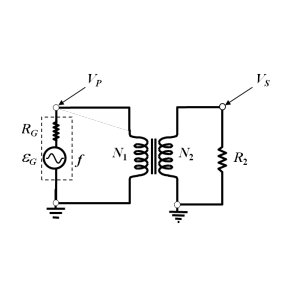
\includegraphics[scale=0.7]{img/transf.jpg}
  \caption{Circuito transformador: Medidas de ganho de tensão e resposta em frequência}
\end{figure}
Para as medidas das tensões primeiramente utilizamos o resistor de $R_{5k}$[\ref{itm:r5k}]. Porém, não conseguimos atingir a tensão máxima de 20.0V, com isso trocamos o resistor pelo $R_{1k}$[\ref{itm:r1k}]. O problema, entretanto, não foi resolvido pois, o último resistor limitava a tensão máxima em $V_{entrada}$ $\approx$ 9.0V, ou seja, o mesmo atuava como um divisor de tensão. Logo, retornamos as medidas utilizando o resistor de valor dado em sala de aula ($R_{5k}$) e variamos $V_{entrada}$ entre 1.0V e 11V. 
\begin{table}
  \tiny
  \centering
  \begin{tabular}{|c|c|c|c|}
    \hline
    $V_{entrada}$ [Volt] & Escala [Volt/div] & $V_{saida}$ [Volt] & Escala [Volt/div]\\
    \hline
    1.06 & 200mili & 3.5 & 500mili\\
2.00 & 500mili & 7.68 & 1\\
3.00 & 500mili & 10.2 & 2\\
4.04 & 1 & 13.80 & 2\\
5.00 & 1 & 17.40 & 5\\
6.00 & 1 & 21.20 & 5\\
8.00 & 2 & 28.40 & 5\\
9.12 & 2 & 32.00 & 5\\
10.10 & 2 & 35.80 & 5\\
11.00 & 2 & 39.6 & 5\\


    
    \hline
  \end{tabular}
  \caption{Tabela de dados $V_{entrada}$ e $V_{saida}$}
\end{table}
Para espiras invertidas, onde $N_{2} < N_{1}$, obtivemos $V_{entrada} = 1.02V (200.0\frac{mV}{div})$ e $V_{saida} = 206.0mV (50,0\frac{mV}{div})$.\\
\subsubsection{Histerese}

\end{document}
